\documentclass[a4paper,man,natbib,floatsintext,donotrepeattitle]{apa6}

\usepackage[english]{babel}
\usepackage[utf8x]{inputenc}
\usepackage{amsmath}
\usepackage{graphicx}
\usepackage[colorinlistoftodos]{todonotes}
\usepackage{xcolor}
\usepackage[draft,inline,nomargin,index]{fixme}
\usepackage{hyperref}
\usepackage{verbatim}
\usepackage{nameref}

\fxsetup{theme=color,mode=multiuser}
\FXRegisterAuthor{ab}{sab}{\color{blue}Amelie} % abnote{} with text inside to edit
\FXRegisterAuthor{bb}{sbb}{\color{purple}Brice} % bbnote{} with text inside to edit
\FXRegisterAuthor{ln}{sln}{\color{violet}Lad} % lnnote{} with text inside to edit

%\title{Blinding as a Necessary Precaution Against Experimenter Biases During Sequential Bayes Factor, comment on "Sequential hypothesis testing with Bayes factors: Efficiently testing mean differences"}

\title{"Efficient" yes, but only if you blind yourself: A commentary on \cite{schonbrodt_sequential_2017}}

%\title{Preventing Possible Biasedness of the Sequential Bayes Factor Design, comment on "Sequential hypothesis testing with Bayes factors: Efficiently testing mean differences"}

\shorttitle{Blind Bayes Factor}
\threeauthors{Amélie G. Bret}{Brice Beffara}{Ladislas Nalborczyk}
\threeaffiliations{Univ. Grenoble Alpes, CNRS, LPNC UMR 5105, F-38000, Grenoble \\Psychological Science Research Institute, Catholic University of Louvain, Belgium}{The Walden III Slowpen Science Laboratory, France}{Univ. Grenoble Alpes, CNRS, LPNC UMR 5105, F-38000, Grenoble \\ Department of Experimental Clinical and Health Psychology, Ghent University}

%\abstract{When collecting data, Bayesian hypothesis testing allows optional stopping with unlimited multiple testing. This procedure is called Sequential Bayes Factor (SBF). Bayes factors are computed until an a priori defined level of evidence is reached. This allows flexible sampling plans and is not dependent upon correct effect size guesses in an a priori power analysis. Testing mean differences between 2 groups, the SBF design typically needs 50\% to 70\% smaller samples to reach a conclusion about the presence of an effect, as compared with optimal NHST, while having the same or lower long-term rate of wrong inference...however... \todo[inline, color=red]{Le début de l'asbtract est extrait de pain joli et al. Il faudra le reformuler.}}

\setcounter{secnumdepth}{3} % re-enabling section numbering (disabled by the apa6.csl)

\begin{document}

% defining a new command for counting words
\newcommand{\quickwordcount}{%
  \immediate\write18{texcount -1 -sum -merge \jobname.tex > \jobname-words.sum }%
  \input{\jobname-words.sum}words%
}

\maketitle

Wordcount: This document contains \textbf{\quickwordcount}.

\newpage

\tableofcontents % provisoire, juste pour se repérer entre nous
\newpage

\section*{TO-DO}

Original papers: \cite{schonbrodt_bayes_2017}, \& \cite{schonbrodt_sequential_2017}...

\begin{itemize}

\item{trouver un acronyme sexy pour décrire le biais, genre le "Sequential Experimenter-Analyst Bias" (SEAB).}

\item{revue de littérature sur le biais de l'expérimentateur, travaux récents ? estimation de la taille d'effet ? \url{https://en.wikipedia.org/wiki/Observer-expectancy_effect}}

\item{répartition des tâches: Lad intro, Brice experimenter biases, Amélie blinding, et tout le monde section 3 et conclusion}

\end{itemize}

%%%%%%%%%%%%%%%%%%%%%%%%%%%%%%%%%%%%%%%%
% début du comment
%%%%%%%%%%%%%%%%%%%%%%%%%%%%%

\newpage

\section{Introduction}

\subsection{Context}

Edwards, Lindman, \& Savage (1963) state, "the rules governing when data collection stops are irrelevant to data interpretation. It is entirely appropriate to collect data until a point has been proven or disproven, or until the data collector runs out of time, money, or patience". However, as noted by \cite{schonbrodt_sequential_2017}, "this practice of unplanned multiple testing is not allowed in the classical NHST paradigm, because it increases Type I error rates (Armitage, McPherson, \& Rowe, 1969). \textit{Of course, one can calculate statistics during data collection, but the results of these tests must not have any influence on optionally stopping data collection}."

In this short commentary, we will argue that such interim analysis (including visual inspections of the data) might have an influence on future data collection through overlooked experimenter biases, thus invalidating the sequential testing procedures (both Bayesian and frequentist). Because we acknowledge and appreciate the huge contribution brought by the original paper of \cite{schonbrodt_sequential_2017}, in the second part of this commentary we consider quick fixes / methodological precautions that will ensure the efficiency of the SBF procedure.

\subsection{the SBF design}

...rosenthal 1963, 1966... as remarked by Wicherts et al. 2015..."It is surprising that blinding to conditions and hypotheses of experimenters, coders, and observers is considered to be crucial during data collection, while in practice, the analyses are typically conducted by a person who is not only aware of the hypotheses, but also benefits directly from corroborating them (commonly by means of a significance test). Together with the many researcher DFs during the analyses, these factors do not entail the most optimal mix for objective and unbiased results.". Moreover, failures to blindings (single, double or triple blind) are three of the QRPs listed by wickerts et al...

\section{SBF problems}

...présenter ici le problème, i.e., le fait que l'échantillonnage soit biaisé: on atteindra plus vite / plus lentement le seuil pré-défini...see Figure \ref{fig:diag1} pour un exemple de ce à quoi je pensais en parlant des diagrammes...created with https://www.draw.io/ ...

...direct consequence of the SEAB is that it introduces a time dependency between participants...this kind of auto-correlated data would be thus better modeled by time-series analyses...

\begin{figure}[H]
  \caption{Overview of the SBF procedure and illustration of possible biases when the experimenter and the data analyst are the same person.}
  \centering
  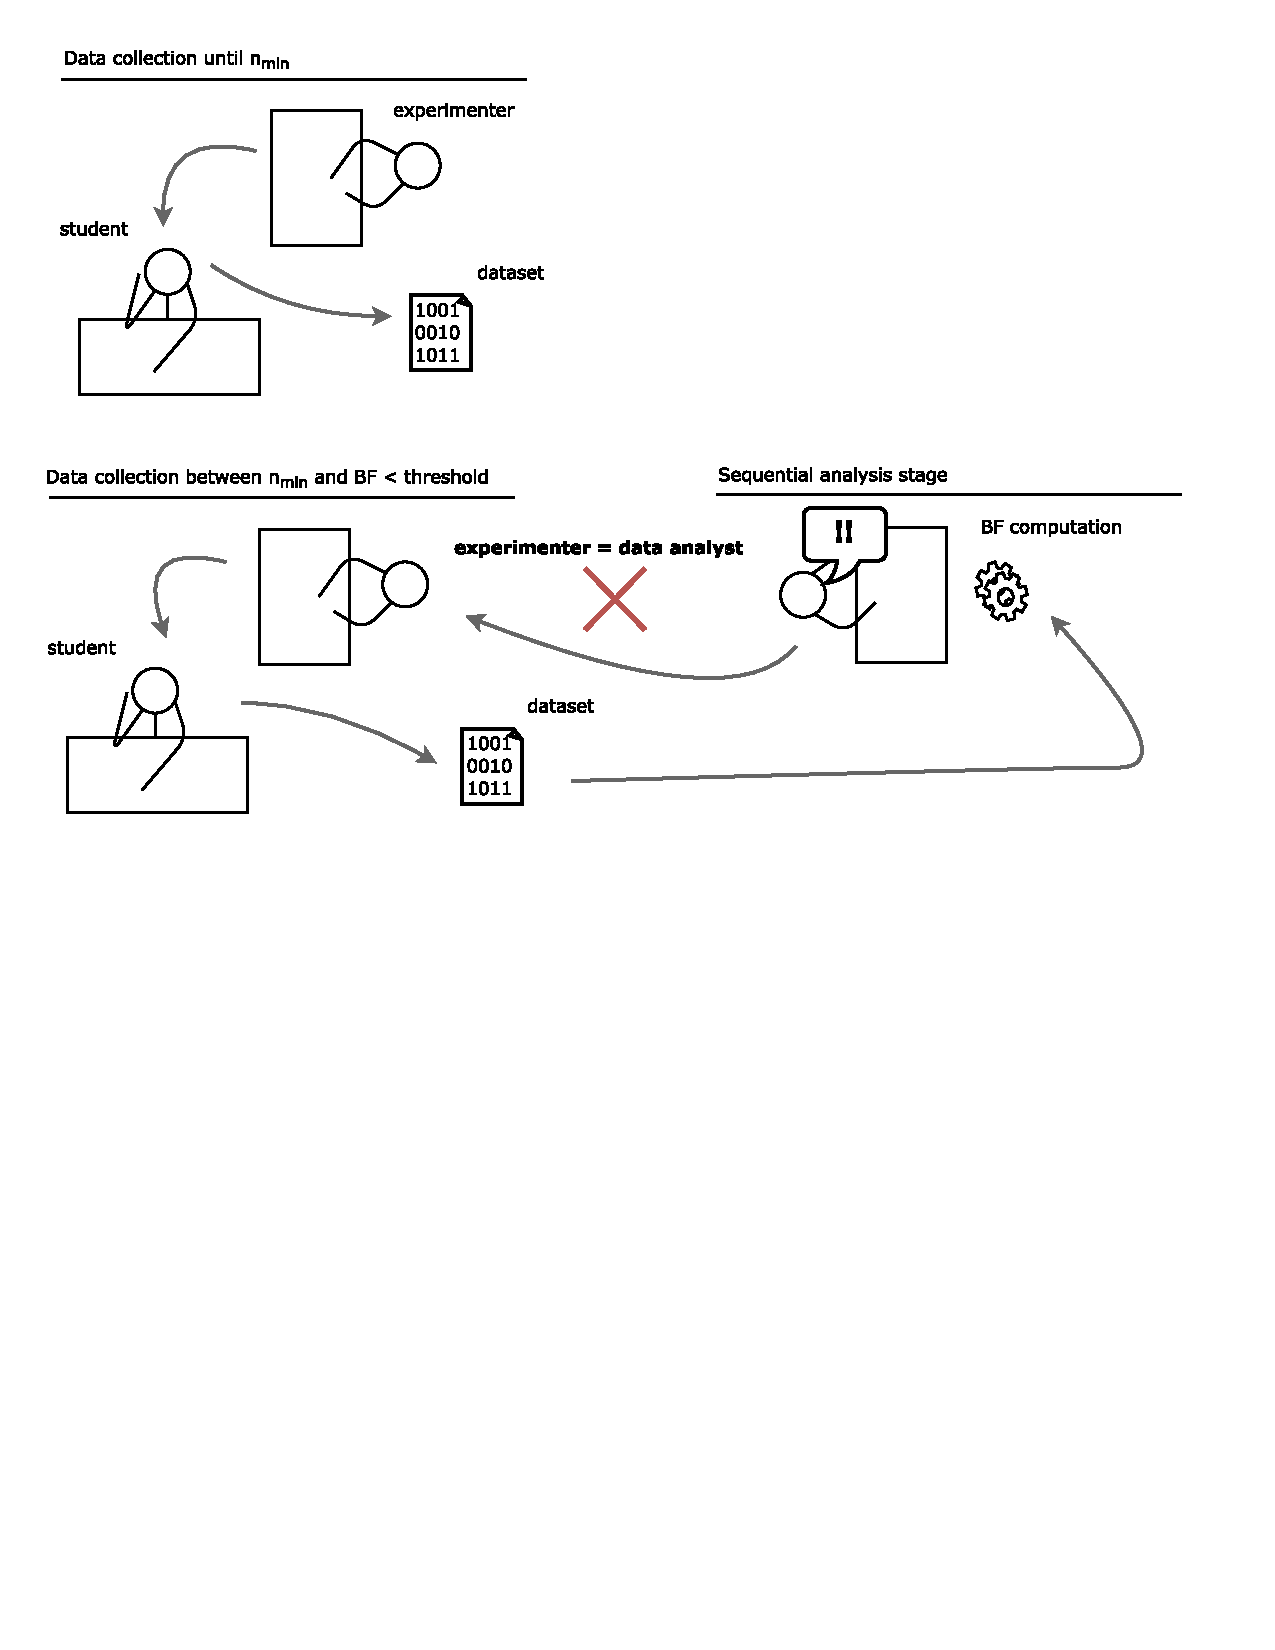
\includegraphics[width=0.8\textwidth]{figures/bias_diag.pdf}
  \label{fig:diag1}
\end{figure}

\section{What does look like SEAB ?}

...the SEAB can wear several forms as we expect different kind of behaviors of the SBF design according to the researcher's "a priori" expectancies and the effect size. Moreover, we focus here on the simplest case in which the expectancies of the researcher are constant throughout the sequential testing. Although non realistic, this setting serves illustrative purposes in the next section.

\subsection{Predictions}

...présenter ici nos prédictions, i.e., ce qu'on s'attend à observer sur l'évolution du SBF dans deux cas (H0 et H1 taille d'effet moyenne, par exemple), selon un chercheur avec des a priori différents...la Figure \ref{fig:pred} illustre nos prédictions pour différents scénarios (e.g., l'expé voit une évolution de BF conforme à ses attentes, non-conforme, etc.)...created with https://www.draw.io/ ...

\begin{figure}[H]
  \caption{Predicted consequences of the SEAB on the results of a SBF procedure, for a given Cohen's d of 0.6 (hereafter, "H1") or of 0 (hereafter "H0"), according to the \emph{a priori} researcher's beliefs.}
  \centering
  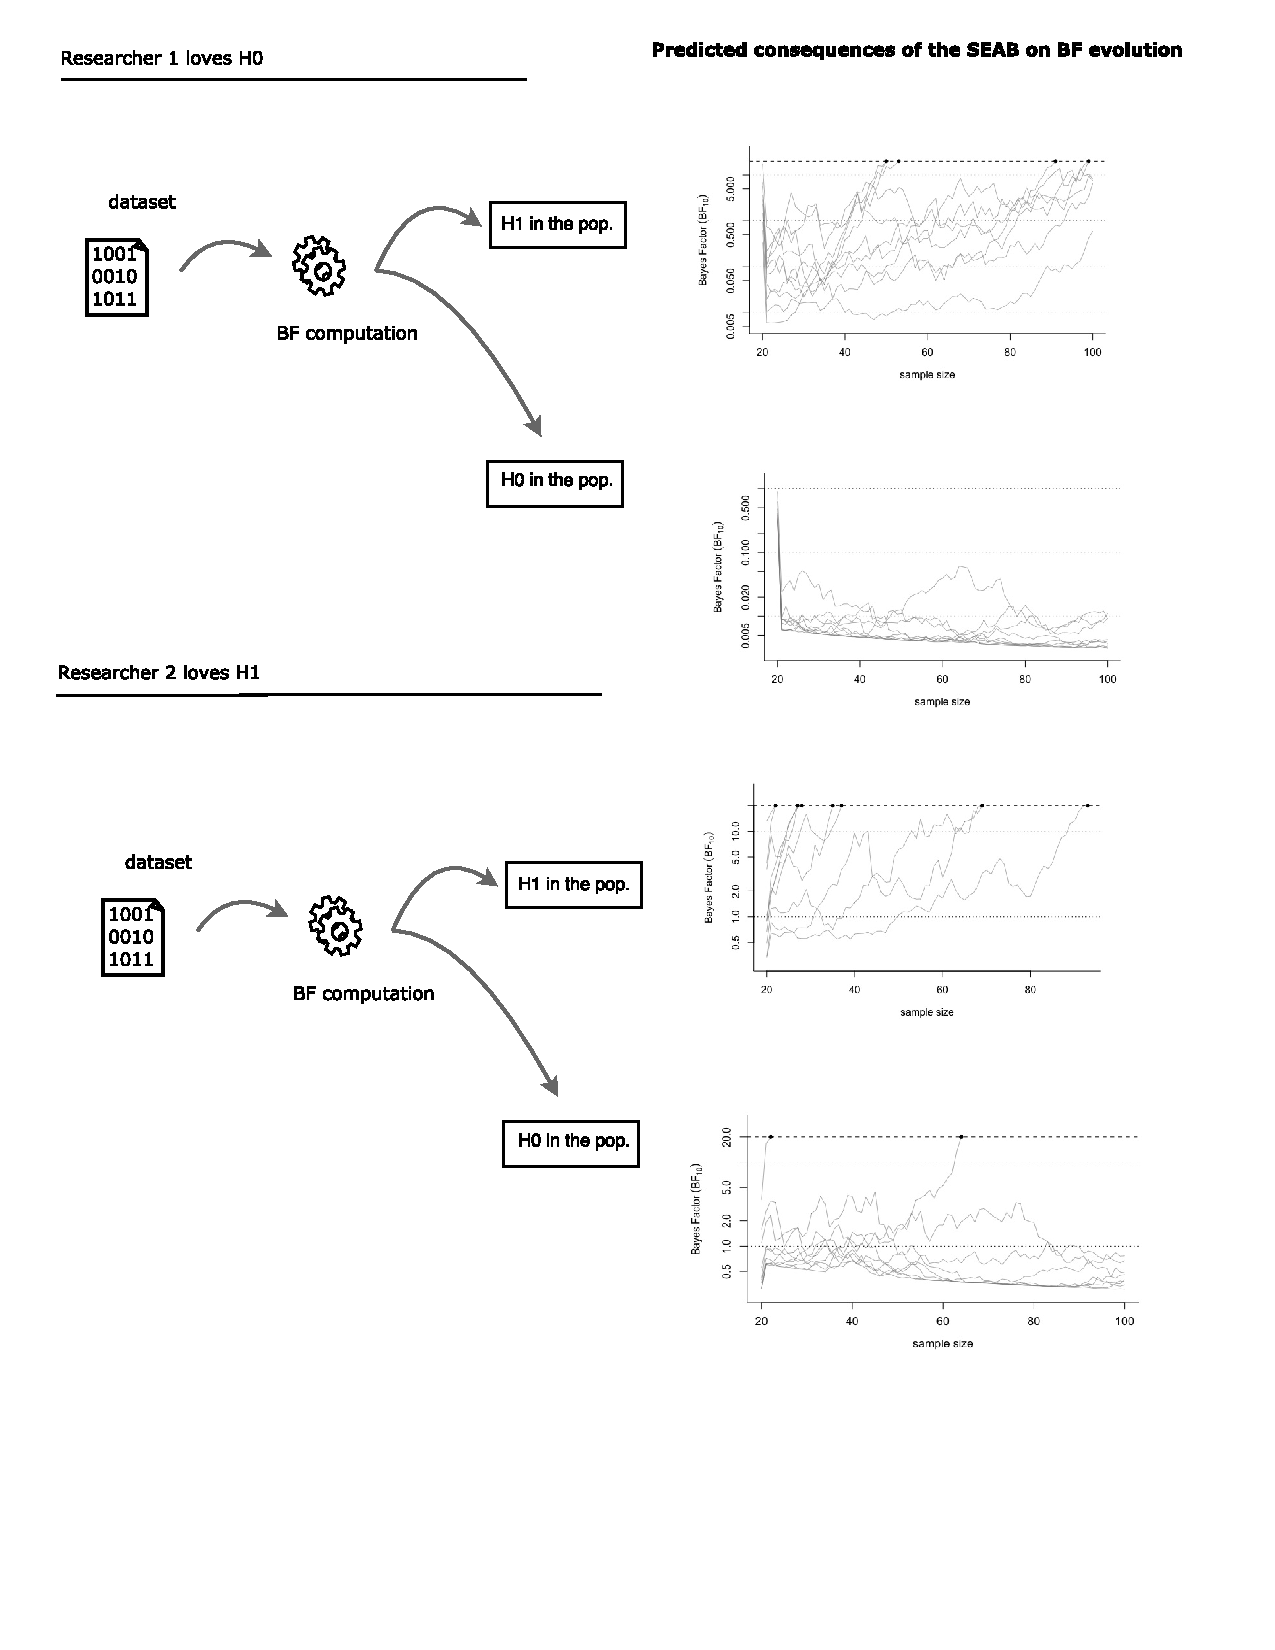
\includegraphics[width=0.8\textwidth]{figures/BFF_predictions.pdf}
  \label{fig:pred}
\end{figure}

\lnnote{peut-être ajouter un plot de l'évolution "normale" du BF pour la même taille d'effet ? et inverser le graphique pour faciliter la comparaison chercheur H0 vs/ chercheur H1}

\subsection{Experimental demonstration}

...proposer ici un protocole expérimental qui permettrait de mettre en évidence le SEAB...

\section{Solutions ? Blind yourself.}

...blinding (double or triple)...

\subsection{Solution 1: one analyst, one experimenter}

...blah blah...

\subsection{Solution 2: one analyst-experimenter, "software-blinded"}

...this solution is relatively costless. To demonstrate this, we added a very short append to the \texttt{seqBF} function, written by Félix Schönbrodt \& Richard Morey (available \href{https://raw.githubusercontent.com/richarddmorey/BayesFactorExtras/master/BayesFactorExtras/R/seqBF.R}{here}), so that the user can now simply set the \texttt{blind} argument to \texttt{TRUE} and thus be completely blind to the results of the sequential BF computations. The only output is a sentence that either indicates to "continue" or to "stop" the recruitment, considering an a-priori defined threshold (see \nameref{sec:supp} for code details).

\section{Conclusions}

...OF COURSE, SEAB can not arise in a context in which double-bliding is efficiently performed...

...exemple de manips utilisant le SBF: \cite{martin_perceiving_2016}...or Matzke, D., Nieuwenhuis, S., van Rijn, H., Slagter, H. A., van der Molen, M. W., \& Wagenmakers, E.-J. (2015). The effect of horizontal eye movements on free recall: A preregistered adversarial collaboration. Journal of Experimental Psychology General, 144, e1–15. http://dx.doi .org/10.1037/xge0000038

\section{Supplementary materials}\label{sec:supp}

...\url{https://github.com/lnalborczyk/Blind_BF}...le repo est privé pour le moment donc on ne peut pas y accéder avec ce lien, mais la fonction est dispo sur le repo Overleaf...

\section{Acknowledgements}

...many thanks to my mom...en plus de ma maman, peut-être faire relire ce commentary par des adultes avant de le soummettre ?...

\bibliography{BBF}

\end{document}
